\documentclass{article}

\usepackage[left=2cm,right=2cm, top=2cm, bottom = 2cm]{geometry}
\usepackage{amsfonts}
\usepackage{amsmath}
%%%\usepackage{array}

\usepackage{tikz}

\pagestyle{empty}

%%%\setlength{\tabcolsep}{1.8cm}
%%%\renewcommand{\arraystretch}{2.5}

%%%\makeatletter
%%%\newcommand{\thickhline}{%
%%%    \noalign {\ifnum 0=`}\fi \hrule height 2pt
%%%    \futurelet \reserved@a \@xhline
%%%}
%%%\newcolumntype{!}{@{\hskip\tabcolsep\vrule width 2pt\hskip\tabcolsep}}
%%%\makeatother

\begin{document}

\title{Plane Polar Coordinates and Inverse Trigonometric Functions}
\date{}

\maketitle
\thispagestyle{empty}

\Large

{\bf \underline{Objective: To understand inverse trig functions and polar}}

{\bf \underline{coordinates, and be able to convert between polar and}}

{\bf \underline{cartesian coordinates.}}

\vspace{5mm}


{\bf Recap of previous material:}

\vspace{5mm}


Consider the diagram below, showing a general point with coordinates $(x,y)$ (pictured here in the third quadrant, but it could be anywhere):

\begin{center}
\begin{tikzpicture}[scale=3]
\draw[->] (-1.5,0) -- (1.5,0);
\node[right] at (1.5,0) {$x$};
\draw[->] (0,-1.5) -- (0,1.5);
\node[above] at (0,1.5) {$y$};

\draw[fill] (-0.707,-0.707) circle [radius=0.05];
\node[above left] at (-0.707,-0.707) {$(x,y)$};

\draw (0,0) -- (-0.707, -0.707);
\node[below right] at (-0.35,-0.35) {$r$};
\draw (0.3,0) arc (0:225:0.3);
\node[above left] at (-0.2,0.2) {$\theta$};

\draw[dashed] (0,-0.707) -- (-0.707,-0.707) -- (-0.707,0);
\end{tikzpicture}
\end{center}



\begin{enumerate}
\item Express the length $r$ from the origin to $(x,y)$ in terms of $x$ and $y$.
\item Express $x$ in terms of $r$ and $\theta$, using a trigonometric function.
\item Express $y$ in terms of $r$ and $\theta$, using a trigonometric function.
\item For the specific point $(-4,2)$, find $r$.
\item For the specific point with $r=2$, $\theta=\frac{4\pi}{3}$, find the $(x,y)$-coordinates. Plot this point on the above diagram.
\end{enumerate}



\clearpage

{\bf Warm-up:}

\vspace{5mm}

\begin{enumerate}
\item What angle does the point $(-1,1)$ make with the positive $x$-axis?
\item What is the distance from the origin to $(-1,1)$?
\item Hence find the point on the unit circle which makes the same angle with the positive $x$-axis as $(-1,1)$.
\item Hence write down an angle $\theta$ such that $\cos(\theta)=\frac{-1}{\sqrt{2}}$ and $\sin(\theta)=\frac{1}{\sqrt{2}}$
\item Is there any other angle $\phi$ such that $\cos(\phi)=\frac{-1}{\sqrt{2}}$?
\item Is there any other angle $\psi$ such that $\sin(\psi)=\frac{1}{\sqrt{2}}$?
\end{enumerate}

\clearpage





{\bf Theory - Inverse Trigonometric Functions:}

\vspace{5mm}

Given any angle $\theta$, we can find $\cos(\theta)$ and $\sin(\theta)$ as the $x$- and $y$-coordinates respectively of the point on the unit circle at angle $\theta$. We can then find $\tan(\theta)$ as the ratio of these two numbers:
\[\tan(\theta)=\frac{\sin(\theta)}{\cos(\theta)}.\]

Can we go the other way? If we know $\sin(\theta)$ and $\cos(\theta)$, we can plot the point with coordinates $(\cos(\theta),\sin(\theta))$, which will lie on the unit circle, and measure the angle it forms with the positive $x$-axis. There are computational methods, such as Newton-Raphson, for figuring out the precise angle $\theta$ without the inaccurate approach of plotting the point and measuring the angle with a protractor.

What if we just know $\sin(\theta)$, without knowing $\cos(\theta)$? Then there are two possible angles $\theta$, because there are two points on the unit circle with the same $y$-coordinate. Similarly, if we know $\cos(\theta)$, there are two points with the same $x$-coordinate, so two possible values of $\theta$. This means that the trigonometric functions \textbf{cannot properly be inverted}.

However, we can partly invert them. The \textbf{inverse trigonometric function} arccos (often denoted $\cos^{-1}$) returns the \textbf{smallest} non-negative angle with a given cosine, always in the range $0\leq\theta\leq\pi$. The inverse trigonometric functions arcsin and arctan (often denoted $\sin^{-1}$ and $\tan^{-1}$ respectively) return the unique angle between $\frac{-\pi}{2}$ and $\frac{\pi}{2}$ having a given sine or tangent respectively.

So $\sin(\sin^{-1}(x))=x$, but $\sin^{-1}(\sin(\theta))$ might not equal $\theta$, but is instead the angle closest to zero with the same sine as $\theta$. Similarly, $\cos(\cos^{-1}(x))=x$, but $\cos^{-1}(\cos(\theta))$ might not equal $\theta$, and $\tan(\tan^{-1}(x))=x$, but $\tan^{-1}(\tan(\theta))$ might not equal $\theta$.

\clearpage


\textbf{Example - arccos:}

\begin{center}
\begin{tikzpicture}[scale=3]
\draw[->] (-1.5,0) -- (1.5,0);
\node[right] at (1.5,0) {$x$};
\draw[->] (0,-1.5) -- (0,1.5);
\node[above] at (0,1.5) {$y$};

\draw[fill,red] (-0.707,-0.707) circle [radius=0.05];
\node[above left, red] at (-0.707,-0.707) {$\left(\frac{-1}{\sqrt{2}},\frac{-1}{\sqrt{2}}\right)$};

\draw[fill,blue] (-0.707,0.707) circle [radius=0.05];
\node[above left, blue] at (-0.707,0.707) {$\left(\frac{-1}{\sqrt{2}},\frac{1}{\sqrt{2}}\right)$};
\draw[blue] (0,0) -- (-0.707,0.707);
\node[blue, left] at (-0.35,0.35) {$1$};

\draw[red] (0,0) -- (-0.707, -0.707);
\node[below right,red] at (-0.35,-0.35) {$1$};
\draw[red] (0.3,0) arc (0:225:0.3);
\node[below left, red] at (0.3,0.3) {$\frac{5\pi}{4}$};

\draw[blue] (0.4,0) arc (0:135:0.4);
\node[blue, above right] at (0.3,0.3) {$\frac{3\pi}{4}$};

%\draw[dashed] (0,-0.707) -- (-0.707,-0.707) -- (-0.707,0);
\end{tikzpicture}
\end{center}


The two points shown both lie on the unit circle and have the same $x$-coordinate, $x=\frac{-1}{\sqrt{2}}$. Therefore
\[\cos\left(\frac{3\pi}{4}\right)=\cos\left(\frac{5\pi}{4}\right)=\frac{-1}{\sqrt{2}}\]
The arccos function returns the smallest non-negative angle having a given cosine, so
\[\cos^{-1}\left(\frac{-1}{\sqrt{2}}\right)=\frac{3\pi}{4}\]



Looking on the graph of the cosine function, we can see the two angles between 0 and $2\pi$ which have cosine $\frac{-1}{\sqrt{2}}$. We also see that there are other angles having the same cosine, because the cos function is $2\pi$-\textbf{periodic}: it repeats exactly every $2\pi$, so $\cos(\theta+2\pi)=\cos(\theta)$.

\begin{center}
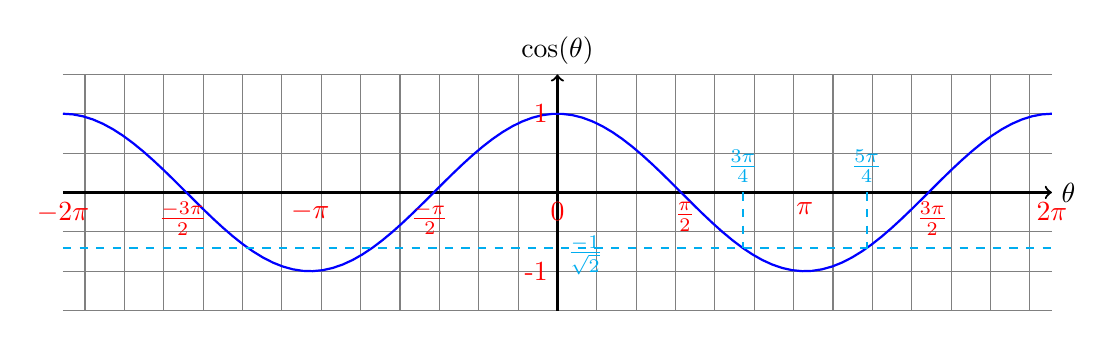
\begin{tikzpicture}
\draw[step=0.5,gray,thin] (-6.28,-1.5) grid (6.28,1.5);
\draw[thick, ->] (0,-1.5) -- (0,1.5);
\node[above] at (0,1.5) {$\cos(\theta)$};
\draw[thick,->] (-6.28,0) -- (6.28,0);
\node[right] at (6.28,0) {$\theta$};

\draw[blue,thick, domain=-6.28:6.28, samples=100] plot (\x,{cos(\x r)});
\node[red,below] at (0,0) {0};
\node[red,below] at (-3.14,0) {$-\pi$};
\node[red,below] at (-1.62,0) {$\frac{-\pi}{2}$};
\node[red,below] at (-4.76,0) {$\frac{-3\pi}{2}$};
\node[red,below] at (-6.28,0) {$-2\pi$};
\node[red,below] at (3.14,0) {$\pi$};
\node[red,below] at (1.62,0) {$\frac{\pi}{2}$};
\node[red,below] at (4.76,0) {$\frac{3\pi}{2}$};
\node[red,below] at (6.28,0) {$2\pi$};
\node[red,left] at (0,1) {1};
\node[red,left] at (0,-1) {-1};

\draw[cyan, thick,dashed] (-6.28,-0.707) -- (6.28, -0.707);
\node[right, cyan] at (0,-0.8) {$\frac{-1}{\sqrt{2}}$};
\draw[cyan,thick,dashed] (2.356,0) -- (2.356,-0.707);
\node[above,cyan] at (2.356,0) {$\frac{3\pi}{4}$};
\draw[cyan,thick,dashed] (3.927,0) -- (3.927,-0.707);
\node[cyan,above] at (3.927,0) {$\frac{5\pi}{4}$};
\end{tikzpicture}
\end{center}


\clearpage


\textbf{Example - arcsin:}

\begin{center}
\begin{tikzpicture}[scale=3]
\draw[->] (-1.5,0) -- (1.5,0);
\node[right] at (1.5,0) {$x$};
\draw[->] (0,-1.5) -- (0,1.5);
\node[above] at (0,1.5) {$y$};

\draw[fill,red] (-0.5,-0.866) circle [radius=0.05];
\node[above left, red] at (-0.5,-0.866) {$\left(\frac{-1}{2},\frac{-\sqrt{3}}{2}\right)$};
\draw[red] (0,0) -- (-0.5, -0.866);
\node[left,red] at (-0.3,-0.35) {$1$};
\draw[red] (0.3,0) arc (0:240:0.3);
\node[below left, red] at (0.3,0.3) {$\frac{4\pi}{3}$};

\draw[fill,blue] (0.5,-0.866) circle [radius=0.05];
\node[above right, blue] at (0.5,-0.866) {$\left(\frac{1}{2},\frac{-\sqrt{3}}{2}\right)$};
\draw[blue] (0,0) -- (0.5,-0.866);
\node[blue, left] at (0.35,-0.35) {$1$};
\draw[blue] (0.4,0) arc (0:300:0.4);
\node[blue, above right] at (0.3,0.3) {$\frac{5\pi}{3}$};

%\draw[dashed] (0,-0.707) -- (-0.707,-0.707) -- (-0.707,0);
\end{tikzpicture}
\end{center}



The two points shown both lie on the unit circle and have the same $y$-coordinate, $y=\frac{-\sqrt{3}}{2}$. Therefore
\[\sin\left(\frac{4\pi}{3}\right)=\sin\left(\frac{5\pi}{3}\right)=\frac{-\sqrt{3}}{2}\]
The arcsin function returns the angle closest to 0 having a given sine, so
\[\sin^{-1}\left(\frac{-\sqrt{3}}{2}\right)=\frac{-\pi}{3}\]
Shifting by $2\pi$ to get a positive angle gives us $\frac{5\pi}{3}$.



Looking on the graph of the sine function, we can see the two angles between 0 and $2\pi$ which have sine $\frac{-\sqrt{3}}{2}$. We also see that there are other angles having the same sine, because the sin function is $2\pi$-\textbf{periodic}: it repeats exactly every $2\pi$, so $\sin(\theta+2\pi)=\sin(\theta)$.


\begin{center}
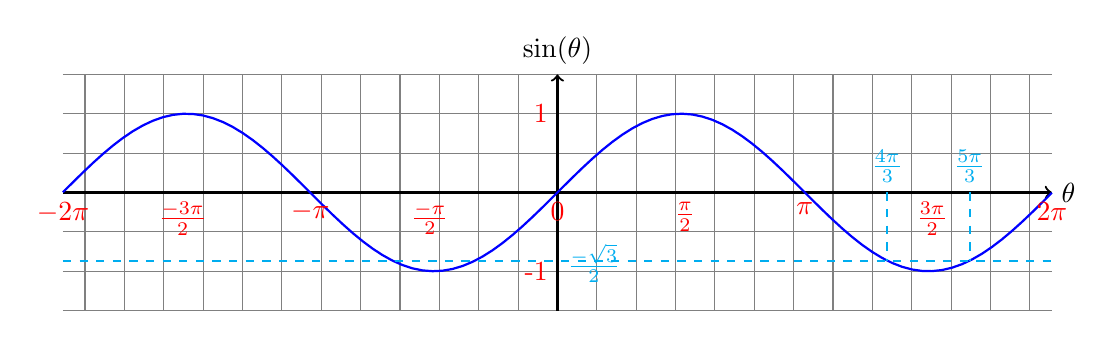
\begin{tikzpicture}
\draw[step=0.5,gray,thin] (-6.28,-1.5) grid (6.28,1.5);
\draw[thick, ->] (0,-1.5) -- (0,1.5);
\node[above] at (0,1.5) {$\sin(\theta)$};
\draw[thick,->] (-6.28,0) -- (6.28,0);
\node[right] at (6.28,0) {$\theta$};

\draw[blue,thick, domain=-6.28:6.28, samples=100] plot (\x,{sin(\x r)});
\node[red,below] at (0,0) {0};
\node[red,below] at (-3.14,0) {$-\pi$};
\node[red,below] at (-1.62,0) {$\frac{-\pi}{2}$};
\node[red,below] at (-4.76,0) {$\frac{-3\pi}{2}$};
\node[red,below] at (-6.28,0) {$-2\pi$};
\node[red,below] at (3.14,0) {$\pi$};
\node[red,below] at (1.62,0) {$\frac{\pi}{2}$};
\node[red,below] at (4.76,0) {$\frac{3\pi}{2}$};
\node[red,below] at (6.28,0) {$2\pi$};
\node[red,left] at (0,1) {1};
\node[red,left] at (0,-1) {-1};

\draw[cyan, thick,dashed] (-6.28,-0.866) -- (6.28, -0.866);
\node[right, cyan] at (0,-0.9) {$\frac{-\sqrt{3}}{2}$};
\draw[cyan,thick,dashed] (4.189,0) -- (4.189,-0.866);
\node[above,cyan] at (4.189,0) {$\frac{4\pi}{3}$};
\draw[cyan,thick,dashed] (5.236,0) -- (5.236,-0.866);
\node[cyan,above] at (5.236,0) {$\frac{5\pi}{3}$};
\end{tikzpicture}
\end{center}





\clearpage


\textbf{Example - arctan:}

Consider the graph of the tangent function, and suppose we want to find angles $\theta$ such that $\tan(\theta)=1$:



\begin{center}
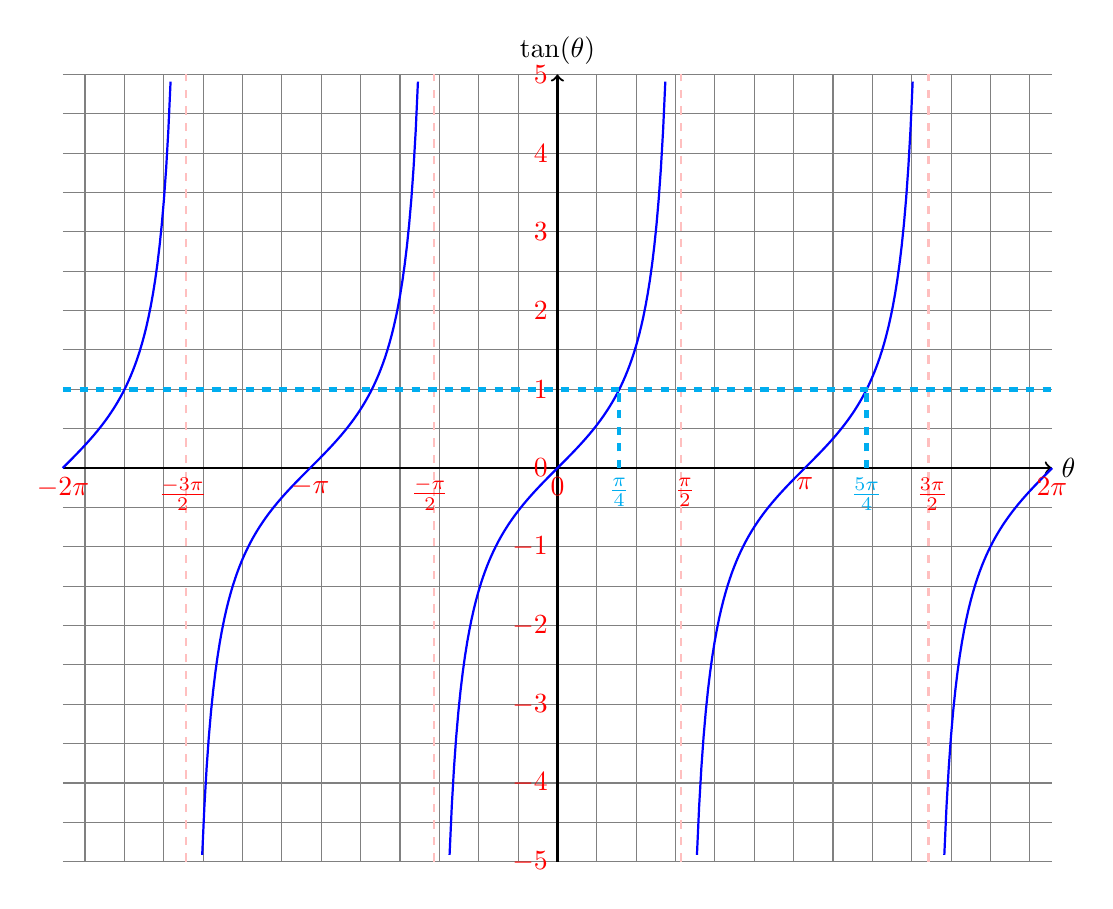
\begin{tikzpicture}
\draw[step=0.5,gray,thin] (-6.28,-5) grid (6.28,5);
\draw[thick, ->] (0,-5) -- (0,5);
\node[above] at (0,5) {$\tan(\theta)$};
\draw[thick,->] (-6.28,0) -- (6.28,0);
\node[right] at (6.28,0) {$\theta$};

\foreach \i in {-1, 0, 1, 2}{
    \pgfmathsetmacro{\start}{\i*pi-1.37}
    \pgfmathsetmacro{\mid}{\i*pi}
    \pgfmathsetmacro{\left}  {(\i-0.5)*pi}
    \draw[dashed, thick,pink] (\left,-5) -- (\left,5); 
    \draw[thick, color=blue] plot [domain=\start:\mid, samples=50] (\x, {tan(\x r)} );
}

\foreach \i in {-2, -1, 0, 1}{
    \pgfmathsetmacro{\mid}{\i*pi}
    \pgfmathsetmacro{\end}  {\i*pi+1.37}
    \draw[thick, color=blue] plot [domain=\mid:\end, samples=50] (\x, {tan(\x r)} );
}


\node[red,below] at (0,0) {0};
\node[red,below] at (-3.14,0) {$-\pi$};
\node[red,below] at (-1.62,0) {$\frac{-\pi}{2}$};
\node[red,below] at (-4.76,0) {$\frac{-3\pi}{2}$};
\node[red,below] at (-6.28,0) {$-2\pi$};
\node[red,below] at (3.14,0) {$\pi$};
\node[red,below] at (1.62,0) {$\frac{\pi}{2}$};
\node[red,below] at (4.76,0) {$\frac{3\pi}{2}$};
\node[red,below] at (6.28,0) {$2\pi$};

\foreach \i in {-5, -4, -3, -2, -1, 0, 1, 2, 3, 4, 5}{
\node[red,left] at (0,\i) {$\i$};
}

\draw[cyan,dashed,ultra thick] (-6.28,1) -- (6.28,1);
\draw[cyan,dashed,ultra thick] (0.785,0) -- (0.785,1);
\draw[cyan,ultra thick,dashed] (3.927,0) -- (3.927,1);
\node[below,cyan] at (0.785,0) {$\frac{\pi}{4}$};
\node[below,cyan] at (3.927,0) {$\frac{5\pi}{4}$};
\end{tikzpicture}
\end{center}


We have that $\tan\left(\frac{\pi}{4}\right)=1$, so $\tan^{-1}(1)=\frac{\pi}{4}$. However, the tan function is $\pi$-periodic (compared with $2\pi$-periodic for sin and cos), so $\tan\left(\frac{5\pi}{4}\right)=1$ also, and, in fact, for any whole number $n$:
\[\tan\left(\frac{\pi}{4}+n\pi\right)=1.\]

So we have seen that for all three trig functions, there are \textbf{infinitely many solutions} $\theta$ to the equation $\sin(\theta)=x$, or $\cos(\theta)=x$, or $\tan(\theta)=x$, and \textbf{two} of these solutions will satisfy $0\leq\theta <2\pi$. Either of these can be the ``correct'' solution to a given problem, so care must be taken to choose the right one. The infinitely many other solutions are just copies of these two as the functions repeat themselves.



\clearpage



\textbf{Practice:}

\vspace{5mm}

\begin{enumerate}
\item $\sin\left(\frac{2\pi}{3}\right)=\frac{\sqrt{3}}{2}$. What is $\sin^{-1}\left(\frac{\sqrt{3}}{2}\right)$?
\item $\cos\left(-\frac{\pi}{4}\right)=\frac{1}{\sqrt{2}}$. What is $\cos^{-1}\left(\frac{1}{\sqrt{2}}\right)$?
\item $\tan(\frac{4\pi}{3})=\sqrt{3}$. What is $\tan^{-1}(\sqrt{3})$?
\end{enumerate}


\clearpage

\textbf{Application: Plane Polar Coordinates:}

\vspace{5mm}

We have seen that if we know the distance $r$ of a point from the origin and the angle $\theta$ that point makes with the positive $x$-axis, we can find the $(x,y)$-coordinates of the point by the formulae
\[x=r\cos(\theta)\qquad y=r\sin(\theta).\]

We have also seen that the distance $r$ can be found by Pythagoras' Theorem:
\[r=\sqrt{x^2+y^2}.\]

Now that we have the inverse trig functions, we can also find $\theta$ from $x$ and $y$. We have:
\begin{align*}
\frac{y}{x}&=\frac{r\sin(\theta)}{r\cos(\theta)}\\
&= \frac{\sin(\theta)}{\cos(\theta)}\\
&=\tan(\theta)
\end{align*}

Now, it \textbf{does not follow} that $\theta=\tan^{-1}(y/x)$, because the arctan function returns the smallest angle having the given tangent. So either $\theta=\tan^{-1}(y/x)$ or $\theta=\pi+\tan^{-1}(y/x)$. We can find which it is by considering whether $x$ and $y$ are positive or negative, and therefore which quadrant the point must lie in.

So given $(x,y)$-coordinates for a point (we call these the \textbf{cartesian coordinates} of the point), we can find $(r,\theta)$-coordinates (we call these \textbf{plane polar coordinates} or just \textbf{polar coordinates}) using
\[r=\sqrt{x^2+y^2}\qquad \tan(\theta)=\frac{y}{x},\]
and given polar coordinates  $(r,\theta)$ for a point, we can find the cartesian coordinates by
\[x=r\cos(\theta)\qquad y=r\sin(\theta).\]
So cartesian and polar coordinates are equivalent ways to describe a point. In some problems, one or other coordinate system makes it easier to find the solution. We will particularly see this when we look at complex numbers and later at calculus.

Note: some people call cartesian coordinates \textbf{rectangular coordinates} instead.

\clearpage



\textbf{Practice:}

\begin{enumerate}
\item Convert the following points from cartesian coordinates to plane polars:
	\begin{enumerate}
	\item $(0,4)$
	\item $(-3,7)$
	\item $(12,-2)$
	\item $(-1,-8)$
	\end{enumerate}
\item Convert the following points from polar coordinates to cartesians:
	\begin{enumerate}
	\item $\left(5,\frac{\pi}{2}\right)$
	\item $(7,3.729)$
	\end{enumerate}
\end{enumerate}





\clearpage


{\bf Key Points to Remember:}

\vspace{5mm}

\begin{enumerate}
\item The \textbf{inverse trigonometric functions} arcsin, arccos, and arctan return the \textbf{angle closest to 0} (and positive for arccos) $\theta$ having a given sine, cosine, or tangent, respectively, but there will be infinitely many other angles possible, and two will lie between 0 and $2\pi$.
\item \textbf{Cartesian coordinates} (or \textbf{rectangular coordinates}) are the usual $(x,y)$-coordinates for describing a point's position.
\item \textbf{Plane polar coordinates} describe a point's position by its distance from the origin $r$ and the angle $\theta$ that it makes with the positive $x$-axis.
\item To convert from polar coordinates to cartesian coordinates, use the formulae:
\[x=r\cos(\theta)\qquad y=r\sin(\theta).\]
\item To convert from cartesian coordinates to polars, use the formulae:
\[r=\sqrt{x^2+y^2}\qquad \tan(\theta)=\frac{y}{x},\]
and consider the quadrant to decide whether
\[\theta=\tan^{-1}\left(\frac{y}{x}\right)\mbox{ or } \pi+\tan^{-1}\left(\frac{y}{x}\right).\]
\end{enumerate}






\end{document}